\begin{questions}
\question{
Radial Functions
}
\begin{solution}
  We know from solving the hydrogen atom that the solutions to the hydrogen atom consist of two parts, the radial and the angular part. For the case when $n=2$ and $l=0,1$ the radial functions are
  \begin{eqnarray}
        R_{20} = \frac{1}{\sqrt{3}}\left(\frac{Z}{2a_0}\right)^{\frac{3}{2}}\left(1- \frac{Zr}{2a_0}\right)e^{-Zr/2a_0},\\
        R_{21} = 2 \left(\frac{Z}{2a_0}\right)^{\frac{3}{2}}\left(\frac{Zr}{a_0}\right)e^{-Zr/2a_0},\qquad
  \end{eqnarray}
  where $a_0$ is the Bohr radius and $Z$ the nuclear charge. If we assume $Z = 1, a_0 =1$ we get the following plot.
\begin{center}
  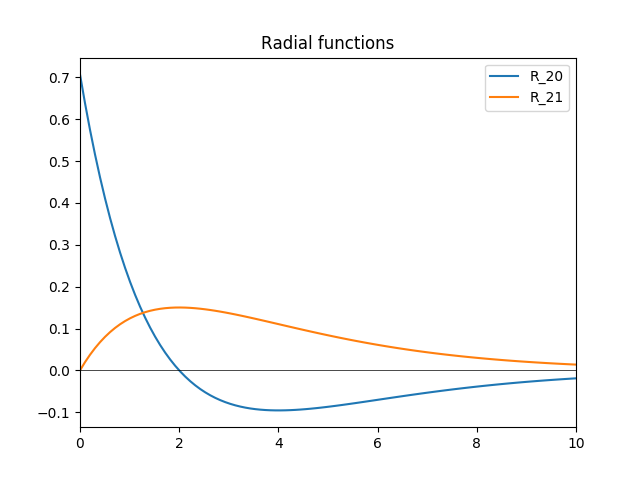
\includegraphics[width=75mm]{radials.png}\label{fig:rad}
  \captionof{figure}{Radial functions $R_{20}$ and $R_{21}$.}
\end{center}
\textbf{How many radial nodes are present?} We don't consider $r=0$ as a node. So taking that in mind, the number of radial nodes will be $n-l-1$, therefore $R_{20}$ must have 1 node and $R_{21}$ none, as we can see in fig. \ref{fig:rad}
\end{solution}

\question{
Qubic Harmonics
}
\begin{solution}

  From previous courses we know how to construct the cubic harmonics with $l=0,1$. By definition

  \begin{eqnarray}
      s = Y_{00}, \qquad \qquad \qquad\label{defs1}\\
      p_z = Y_{10} \qquad \qquad \qquad\label{defs2}\\
      p_x= \sqrt{\frac{1}{2}}(Y_{1-1} - Y_{11}),\label{defs3}\\
      p_y = \sqrt{\frac{1}{2}}i(Y_{1-1} + Y_{11}),
      \label{defs4}
  \end{eqnarray}

  The spherical harmonics for $l=0,1$ are

  \begin{eqnarray}
      Y_{00} = \sqrt{\frac{3}{4\pi}}, \qquad \qquad \quad \label{y00}\\
      Y_{10} = \sqrt{\frac{3}{4\pi}}\cos{\theta}, \qquad \quad \label{y10}\\
      Y_{1\pm1}= \mp \sqrt{\frac{3}{8\pi}}\sin{\theta}e^{\pm i\phi}, \label{y11}
  \end{eqnarray}

  Plugging eqs. \ref{y00}-\ref{y11} into eqs. \ref{defs1}-\ref{defs2} yields,

  \begin{eqnarray}
      \hlgreen{s = \sqrt{\frac{3}{4\pi}},} \qquad \quad \quad\\
      \hlgreen{p_z = \sqrt{\frac{3}{4\pi}}\cos{\theta},} \qquad\\
      \hlgreen{p_x= \sqrt{\frac{3}{4\pi}}\sin{\theta}\cos{\phi},}\\
      \hlgreen{p_y = \sqrt{\frac{3}{4\pi}}\sin{\theta}\sin{\phi}.}
  \end{eqnarray}

  Now from this and our knowledge that the wavefunctions are given by

  \begin{equation}
    \psi_{nlm}(\vec{r}) =A R_{nl}(r)h_{l\alpha}(\theta,\phi),
  \end{equation}
  we must be able to complete this exercise.

  \textbf{How do the wavefunctions look like for $n=2,l=0$ and $n=2,l=1$ ?}

  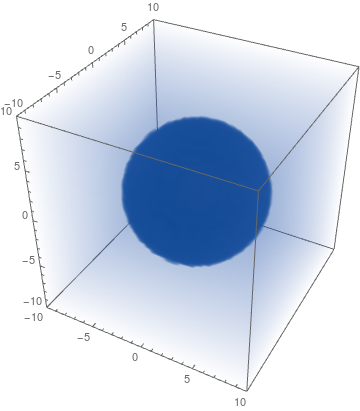
\includegraphics[width=37mm]{s.png}
  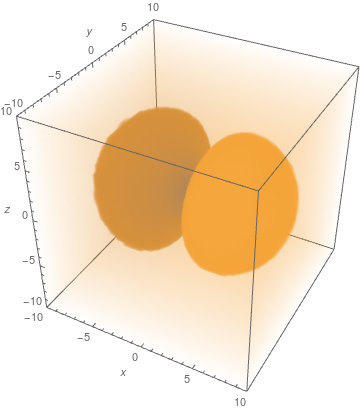
\includegraphics[width=37mm]{px_3d.png}
  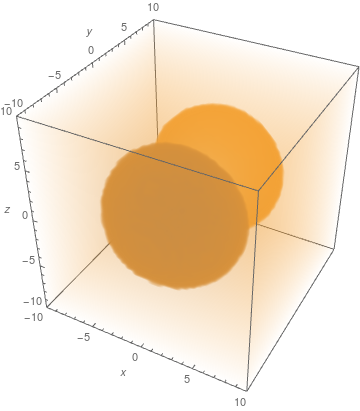
\includegraphics[width=37mm]{py_3d.png}
  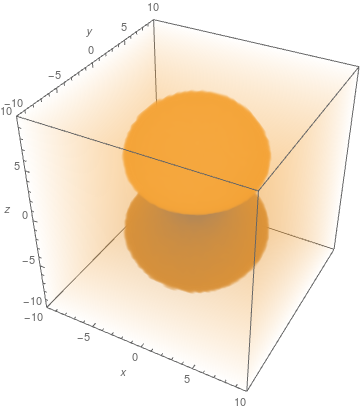
\includegraphics[width=37mm]{pz_3d.png}\label{fig:3d}

  \hspace{1.7cm}a)\hspace{35mm}b)\hspace{35mm}c)\hspace{35mm}d)
  \captionof{figure}{3D plots for the wavefunctions $\psi_{200}$,  $\psi_{21x}$, $\psi_{21y}$, $\psi_{21z}$, from a) to b) respectively.}
  \vspace{0.5cm}
  Here we can see that the p functions consist of two lobes with different sign each.\clearpage

  \textbf{Draw contour plots on the xy plane}

  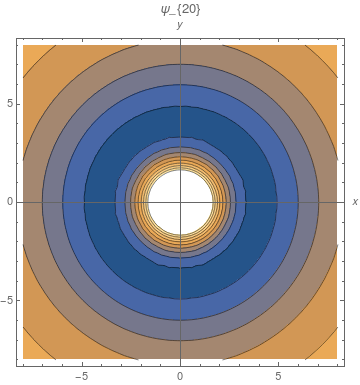
\includegraphics[width=37mm]{cont_s.png}
  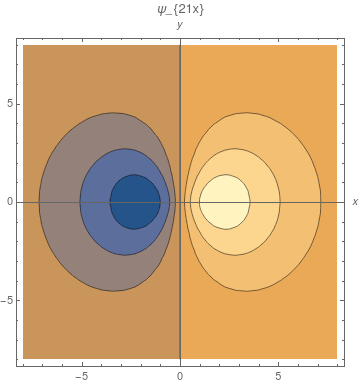
\includegraphics[width=37mm]{cont_px.png}
  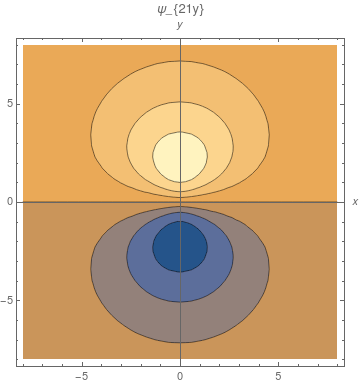
\includegraphics[width=37mm]{cont_py.png}
  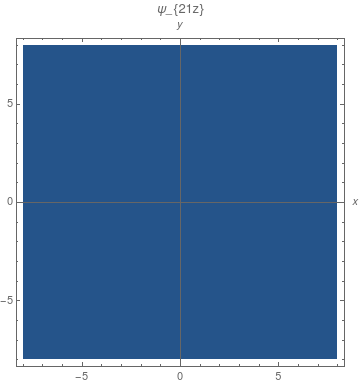
\includegraphics[width=37mm]{cont_pz.png}\label{fig:cont}

  \hspace{1.7cm}a)\hspace{35mm}b)\hspace{35mm}c)\hspace{35mm}d)
  \captionof{figure}{Contour plots on the $xy$ plane for the wavefunctions $\psi_{200}$,  $\psi_{21x}$, $\psi_{21y}$, $\psi_{21z}$, from a) to b) respectively.}
\vspace{0.5cm}
  \textbf{Which functions have inversion symmetry?}
  If we don't consider signs only $\psi_{200}$ has inversion symmetry. But if we are not that rigorous and we allow ourselves to take the absolute value of the functions then all of them have inversion symmetry with respect to the origin.
\end{solution}
\end{questions}


% \includegraphics[width=75mm]{}\label{}
%
%
%  \captionof{figure}{}
